\documentclass[border=10pt]{standalone}
\usepackage{tikz}
\usetikzlibrary{arrows.meta}

\definecolor{shapegray}{RGB}{160,160,160}
\definecolor{shapedark}{RGB}{110,110,110}
\definecolor{arrowred}{HTML}{a00000}

\begin{document}
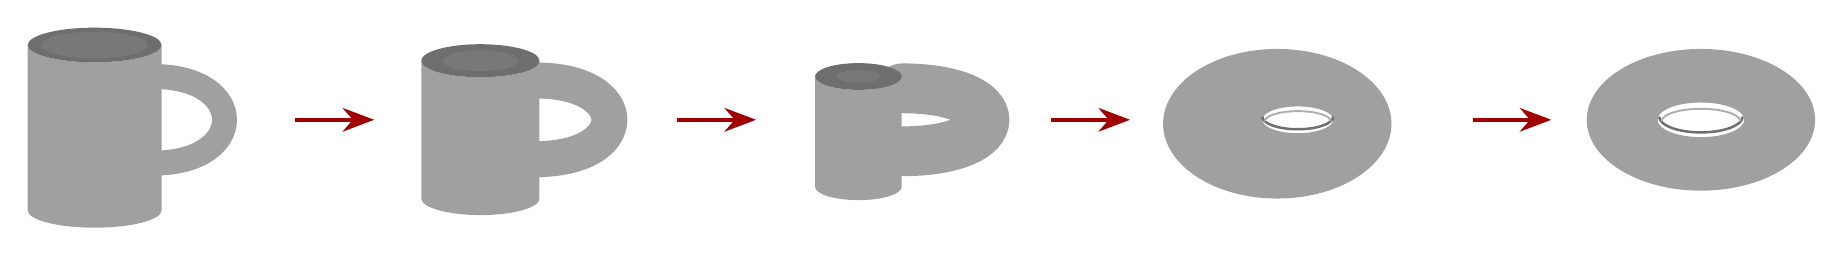
\begin{tikzpicture}[
    arrow/.style={
        -{Stealth[length=4mm, width=3mm]},
        line width=1.4pt,
        draw=arrowred
    }
]

% =================== Stage 1: Coffee Mug ===================
\begin{scope}[shift={(0,0)}]
    \draw[shapegray, line width=9pt, line cap=round]
        (0.75, 0.55) .. controls (1.95, 0.55) and (1.95, -0.55) .. (0.75,-0.55);
    \fill[shapegray]
        (-0.85,-1.15)
        -- (-0.85, 0.95)
        arc[start angle=180, end angle=360, x radius=0.85, y radius=0.22]
        -- (0.85,-1.15)
        arc[start angle=0, end angle=-180, x radius=0.85, y radius=0.22]
        -- cycle;
    \fill[shapedark] (0, 0.95) ellipse[x radius=0.85, y radius=0.22];
    \fill[shapegray!75!black] (0, 0.95) ellipse[x radius=0.68, y radius=0.17];
\end{scope}

% Arrow 1
\draw[arrow] (2.55, 0) -- (3.55, 0);

% =================== Stage 2: Shallower mug, thicker handle ===================
\begin{scope}[shift={(4.9,0)}]
    \draw[shapegray, line width=13pt, line cap=round]
        (0.70, 0.50) .. controls (1.95, 0.50) and (1.95, -0.50) .. (0.70,-0.50);
    \fill[shapegray]
        (-0.75,-1.00)
        -- (-0.75, 0.75)
        arc[start angle=180, end angle=360, x radius=0.75, y radius=0.21]
        -- (0.75,-1.00)
        arc[start angle=0, end angle=-180, x radius=0.75, y radius=0.21]
        -- cycle;
    \fill[shapedark] (0, 0.75) ellipse[x radius=0.75, y radius=0.21];
    \fill[shapegray!75!black] (0, 0.75) ellipse[x radius=0.48, y radius=0.13];
\end{scope}

% Arrow 2
\draw[arrow] (7.40, 0) -- (8.40, 0);

% =================== Stage 3: Stub body, fat handle ===================
\begin{scope}[shift={(9.7,0)}]
    \draw[shapegray, line width=18pt, line cap=round]
        (0.55, 0.40) .. controls (1.95, 0.40) and (1.95, -0.40) .. (0.55,-0.40);
    \fill[shapegray]
        (-0.55,-0.85)
        -- (-0.55, 0.55)
        arc[start angle=180, end angle=360, x radius=0.55, y radius=0.17]
        -- (0.55,-0.85)
        arc[start angle=0, end angle=-180, x radius=0.55, y radius=0.17]
        -- cycle;
    \fill[shapedark] (0, 0.55) ellipse[x radius=0.55, y radius=0.17];
    \fill[shapegray!75!black] (0, 0.55) ellipse[x radius=0.28, y radius=0.08];
\end{scope}

% Arrow 3
\draw[arrow] (12.15, 0) -- (13.15, 0);

% =================== Stage 4: Asymmetric torus (body absorbed) ===================
\begin{scope}[shift={(15.1,0)}]
    \fill[shapegray, even odd rule]
        (-0.08, -0.05) ellipse[x radius=1.45, y radius=0.95]
        (0.18, 0) ellipse[x radius=0.45, y radius=0.17];
    \draw[shapedark, line width=0.9pt]
        (-0.27, 0.04) arc[start angle=180, end angle=360, x radius=0.45, y radius=0.16];
    \draw[shapegray!85!white, line width=0.7pt]
        (-0.24, -0.02) arc[start angle=180, end angle=0, x radius=0.42, y radius=0.13];
\end{scope}

% Arrow 4
\draw[arrow] (17.50, 0) -- (18.50, 0);

% =================== Stage 5: Donut / Torus ===================
\begin{scope}[shift={(20.40,0)}]
    \fill[shapegray, even odd rule]
        (0,0) ellipse[x radius=1.45, y radius=0.90]
        (0,0) ellipse[x radius=0.55, y radius=0.22];
    \draw[shapedark, line width=0.9pt]
        (-0.53, 0.04) arc[start angle=180, end angle=360, x radius=0.53, y radius=0.20];
    \draw[shapegray!85!white, line width=0.7pt]
        (-0.50, -0.02) arc[start angle=180, end angle=0, x radius=0.50, y radius=0.16];
\end{scope}

\end{tikzpicture}
\end{document}
